\section{Segregacja krzywych dyspersji}
Kod odpowiedzialny za segregację krzywych dyspersji wygenerowanych z solvera opisanego w poprzedniej sekcji znajduje się w pliku selectMode.py w katalogu o nazwie Propagation. Jego miejsce w drzewie projektu przedstawia rysunek \ref{fig:gdzie jest select}
\begin{figure}[h]
\centering
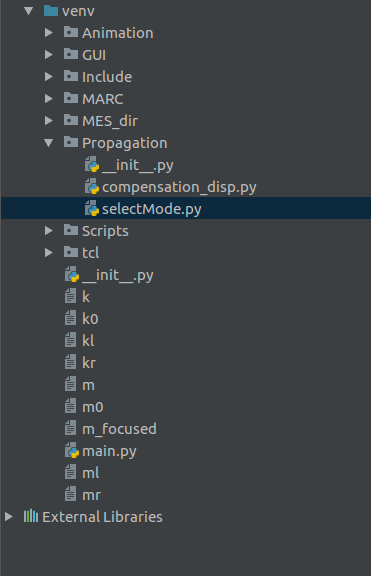
\includegraphics[width=10cm]{Zdjecia/5/kasia/selectMode}
\caption{Lokalizacja pliku selectMode.py w drzewie projektu}
\label{fig:gdzie jest select}
\end{figure}
Jest to jedyna część aplikacji napisana całkowicie obiektowo. Zastosowanie programowania obiektowego w przypadku tej części aplikacji znacząco ułatwiło późniejsze używanie stworzonego rozwiązania jak i uporządkowało sam kod. Plik selectMode został stworzony aby w sposób łatwy i szybki można było przeprowadzić agregacją punktów do konkretnych krzywych dyspersji a następnie w sposób łatwy i intuicyjny z nich korzystać. Samo generowanie obiektu przechowującego wszystkie krzywe dyspersji jest bardzo łatwe. Należy najpierw stworzyć obiekt typu SelectMode, jako argumenty podając ścieżki względne kolejno do pliku kvect oraz omega. Następnie należy wywołać metodę stworzonego właśnie obiektu o nazwie selectMode(). Od tego momentu nasz obiekt przechowuje posortowane krzywe dyspersji.

Podstawową jednostką są tu obiekty klasy Point. Klasa ta jak wszystkie omawiane w tej sekcji znajduje się w pliku selctMode.py. Klasa ta posiada jedynie konstruktor, przyjmujący dwa parametry: w,k. Obiekt ten reprezentuje pojedynczy punkt wygenerowany przez zaimplementowany solver MES. Wartość w jest wartością zespoloną i odpowiada wartości znajdującej się na osi x wykresu krzywej dyspersji, czyli częstości kątowej, natomiast k odpowiada wartości y tego wykresu i oznacza liczbę falową. Obydwa parametry przyjmują wartości domyślne wynoszące zero. Klasa ta ma cztery pola:

$w$ - przechowujące wartość częstotliwości w kHz

$wkat_real_part$ - przechodujące część rzeczywistą podanej do konstruktora częstości

$wkat_complex$ - przechowujące zespoloną częstość kątową podaną do konstruktora

$k$ - przechowujące wartość liczby falowej podaną do konstruktora.

Klasa ta posiada tylko jedną metodę:

$printCoor()$, która nie przyjmuje żadnych argumentów. Jej funkcją jest wypisywanie w konsoli współrzędnych punktu w postaci: "w=[wartość w kHz], k=[wartość w rad/m]"

Kolejną, bardziej złożoną klasą, wykorzystywaną do przechowywania krzywych dyspersji jest klasa $Mode$. Jej głównym zadaniem jest przechowywanie zbioru punktów. Posiada konstruktor bezparametrowy oraz następujące pola:

$points$ - tablica przechowująca zbiór punktów, domyślnie pusta

$minOmega$ - minimalna przechowywana wartość $\omega$ wyrażona w kHz, póki tablica $points$ jest pusta przyjmuje wartość $float('inf')$

$min_omega_kat$ = minimalna przechowywana wartość $\omega$ wyrażona w $\frac{rad}{s}$, póki tablica $points$ jest pusta przyjmuje wartość $float('inf')$

$allOmega$ - tablica przechowująca wartości wszystkich częstotliwości w postaci zespolonej, domyślnie pusta

$all_omega_khz$ - tablica przechowująca wartości wszystkich częstotliwości w kHz, domyślnie pusta

Klasa ta ma zaimplementowane następujące metody:

$addPoint$ funkcja ta przyjmuje jeden parametr. Jest nim obiekt klasy Point. Dodaje ona punkt do listy punktów ($self.points$), list $self.allOmega$ i $self.all)omega)khz$ oraz, jeśli to konieczne ustawia wartości pól $self.min_omega_kat$ oraz $minOmega$.

$delPoint$ funkcja analogiczna znaczeniowo do $self.addPoint$, jako parametr przyjmuje obiekt klasy Point. Podany punkt jest wyszukiwany w tablicy $self.points$ a następnie usuwany.

$delDuplicats$ funkcja przyjmująca jako argument tablice obiektów typu Point. Jej zadaniem jest usunięcie z tablisy $self.points$ wszystkich punktów z podanej listy.

$quicksort$ to funkcja przyjmująca dwa parametry, indeks początkowy i końcowy. Jej zadaniem jest posortowanie przechowywanych punktów rosnąco względem częstości kątowych. Argument $pocz$ oznacza początkowy indeks tablicy, natomiast $koniec$ indeks końcowy. Jest to funkcja działająca rekurencyjnie. Zasada działania tego sortowania opiera się na metodzie "dziel i zwyciężaj", której główną zasadą jest rozbijanie dużego problemu na skończoną ilość mniejszych podproblemów tak długo, aż staną się one trywialne do rozwiązania. W tym przypadku wybiera się tak zwany piwot wokół którego rozdziela się elementy do lewej i prawej tablicy. W lewej znajdują się elementy mniejsze w prawej większe. W ten sposób piwot znajduje sia na swoim właściwym miejscu. Natomiast na lewej i prawe tablicy znów wywołuje się metode quicksort. Postępuje się w ten sposób aż do uzyskania tablic jednoelementowych, które są już posortowane. Jest to bardzo dobry algorytm, zwłaszcza do sortowania dużej ilości danych.

$findAngle$ to funkcja przyjmująca jeden parametr - obiekt typu Point. Ma ona za zadanie wyznaczyć kąt pomiędzy dwoma wektorami. Pierwszy z nich stworzony jest przez dwa ostatnie punkty w tablicy $self.points$ drugi natomiast to wektor mający początek w ostatnie punkcie tablicy $self.point$ natomiast koniec w podanym w argumencie punkcie. Do obliczenia szukanego kąta wykorzystywana jest następująca zależność:
\begin{equation}
cos \alpha = \frac{a \circ b}{|a|\cdot |b|}
\end{equation}
\begin{equation}
\alpha = arccos \frac{a \circ b}{|a|\cdot |b|}
\end{equation}

Gdzie:
$a \circ b$ - oznacza iloczyn skalarny wektorów a i b

$|a|,|b|$ - oznacza długość tych wektorów

Funkcja zwraca wartość tak obliczonego kąta.

$findSmallestAngle$ jest funkcją przyjmującą dwa argumenty. Pierwszy z nich to jednowymiarowa tablica obiektów klasy Point, natomiast drugi do odległość wyrażona w kHz, w jakiej mają znajdować się brane pod uwagę punkty. Funkcja bierze wszystkie punkty z podanej listy i wybiera spośród nich ten, który tworzy najmniejszy kąt z wektorem stworzonym z dwóch ostatnich punktów. Brane pod uwagę są tylko te punkty, które znajdują się odpowiednio blisko ostatniego punktu listy $self.points$. wartość drugiego parametru jest ustawiona na domyślną. Jeśli w trakcie przeszukiwania danej tablicy punktów okazałoby się, że nie ma punktu w wyznaczonym otoczeniu, funkcja wywoływana jest rekurencyjnie z odpowiednio powiększonym zakresem otoczenia. Wartość zwracana to indeks punktu, najlepiej pasującego do już istniejącego zbioru punktów. Funkcja ta jest wykorzystywana bezpośrednio do segregacji krzywych dyspersji. Znalezienie punktu najbardziej odpowiadającego już istniejącej krzywej, a co za tym idzie tworzącego najmniejszy kąt i znajdującego się w odpowiednim sąsiedztwie jest kluczowym zadaniem pozwalającym na segregację punktów.

$findPointWithK$ przyjmuje jeden argument, k. Wyszukuje w tablicy $self.points$ wszystkie punkty, których wartość pola k jest równa zadanej wartości. Zwraca tablicę tych punktów.

$findPoint$ przyjmuje dwa argumenty: points i omega. Points to dwuelementowa tablica zawierająca obiekty klasy Point. Funkcja na podstawie podanych dwóch punktów interpoluje prostą iraz zwraca wartość tej prostej w punkcie omega.

$findPointWithGivenK$ przyjmuje dwa argument: points oraz k. działa analogicznie do funkcj $self.findPoin$ lecz zamiast zwracać wartość funkcji na podstawie jej argumentu, zwraca argument na podstawie podanej wartości k, zwracana wartość wyrazona jest w kHz.

$findPointWithGivenK_rad_s$ ta funkcja również przyjmuje dwa argumenty, a jej działanie jest identyczne jak działanie funkcji self.findPointWithGivenK, z tą różnicą, iż zwracany wynik wyrażony jest w $\frac{rad}{s}$

$findKWithGivenOmega_kHz$ przyjmuje jeden parametr, omega, będący częstotliwością wyrażoną w kHz. Oblicza wartość przechowywanej krzywej dyspersji dla podanej częstotliwości. Zwraca liczbę falową odpowiadającą podanej omedze.

Klasa Mode wykorzystywana jest zarówno do przechowywania zbioru punktów (na początek przechowuje cały zbiór wygenerowanych przez solver punktów), jak również na późniejszym etapie obiekty typu Mode przechowują pojedyncze krzywe dyspersji.

Kolejną klasą w stworzonej strukturze jest klasa Data. Posiada ona konstruktor bezparametrowy oraz jedno pole:

$modeTable$ - jest to tablica przechowująca obiekty typu Mode, przechowujące punkty należące do kolejnych krzywych dyspersji.

Klasa ta posiada również jedną metodę:

$addMode$ - przyjmuje obiekt typu mode i dodaje go do tablicy $self.modeTable$

Najbardziej nadrzędną klasą jest klasa SelectMode. Posiada ona konstruktor przyjmujący trzy parametry: 

$kvect_path$ - ścieżka do wygenerowanego przez solver pliku kvect, 

$omega_path$ - ścieżka do wygenerowanego przez solver pliku omega, 

$rows$ - liczba kolumn w pliku omega, które chcemy wczytać, domyślnie ustawiona na cały plik czyli 426 kolumn.

Klasa ta posiada 5 pól. Są to:

$eig_path$ - przechowująca podaną ścieżkę do pliku kvect

$omega_path$ - przechowująca podaną ściężkę do pliku omega

$rows$ - przechowująca liczbę kolumn do odczytu

$AllModes$ - obiekt typu Data. Na poczatku nie przechowujący żadnych danych

$k_v$ - wektor wartości liczby falowej. Domyślnie pusty

W klasie tej zostały zaimplementowane trzy metody:

$getMode$, która jako argument przujmuje liczbę całkowitą, natomiast zwraca obiekt typu Mode. Jej zadaniem jest z obiektu przechowującego wszystkie krzywe dyspersji, wybrać tę o podanym numerze i zwrócić ją w postaci obiektu klasy Mode.

$plot_modes$, która jako argument przyjmuje tablice liczb całkowitych będących indeksami krzywych, które chcemy wyświetlić. Ta funkcja niczego nie zwraca, jedynie generuje wykres żądanych krzywych dyspersji.

$selectMode$ jest funkcją nie przyjmującą żadnych parametrów. Na podstawie podanych do konstruktora danych wczytuje wektor liczb falowych z pliku kvect. następnie tworzy obiekt typu Mode,$AllPoints$, do którego następnie wczytuje wszystkie punkty wygenerowane przez solver. Następnie tworzone są dwa obiekty klasy Mode: $MinKTable$ oraz $MinKTable2$ Pierwsza z nich przechowuje punkty o wartości k równej najmniejszej wartości występującej w wektorze liczb falowych, natomiast druga przechowuje punkty, których wartość liczby falowej jest drugą najmniejszą wartością z wektora liczb falowych.

Te wybrane punkty, uszeregowane względem omeg stanowią zestaw dwóch pierwszych punktów kolejnych krzywych dyspersji. Następnym krokiem jest usunięcie ich z wektora $self.AllPoints$. Ostatnim etapem segregacji jest wybieranie kolejnych punktów z wektora $self.AllPoints$ o aktualnie najniższej wartości liczby falowej, oraz przydzielanie ich do odpowiednich modów, używając funkcji $findSmallestAngle$. Wszystkie przydzielone punkty są usuwane z wektora $self.AllPoints$. Procedura jest powtarzana do momentu aż wektor ten stanie się pusty.

Listing przykładowego kodu, agregującego punkty do krzywych dyspersji, oraz rysowania wybranej krzywej:

$Mody = SelectedMode('../eig/kvect', '../eig/omega')$

$Mody.selectMode()$

$Mody.plot_modes(50)$

